\documentclass[11pt]{article}

\usepackage[margin=1in]{geometry}
\usepackage{graphicx}
\usepackage{booktabs}
\usepackage{amsmath,amssymb}
\usepackage{hyperref}
\usepackage{xcolor}
\usepackage{microtype}
\usepackage{authblk}
\usepackage[numbers,sort&compress]{natbib}

\title{Network Statistics of the Whole-Brain Connectome of \textit{Drosophila}}
\author{FlyWire Consortium network-analysis team}
\date{}

\begin{document}
\maketitle

\begin{abstract}
Whole-brain connectomes at synaptic resolution offer an unprecedented
opportunity to uncover the organizational principles of neural networks, but
large-scale topological analyses across sensory, associative, and motor
regions have until now been limited by dataset size and completeness. Here
we exploit the FlyWire v630 synapse-resolution reconstruction of the adult
\textit{Drosophila melanogaster} brain---containing $127{,}978$ neurons and
$2{,}613{,}129$ connections after thresholding at five synapses per
connection---to compute global network statistics, connected-component
structure, rich-club coefficients, two- and three-node motif frequencies
with neurotransmitter composition, and subnetwork properties within the 78
anatomically defined neuropils of the brain. We benchmark every metric
against directed Erd{\H o}s--R{\'e}nyi, configuration, and two-zone spatial
null models. The brain forms a single giant strongly connected component
containing 93.3\% of neurons and a giant weakly connected component
containing 98.8\%. It harbors a large rich club of $40{,}218$ neurons
(approximately 30\% of the connectome), whose internal connection
probability of $0.000870$ is 5.4 times the brain-wide value of $0.000161$.
Reciprocity ($0.138$) and clustering ($0.0463$) exceed all three null models;
feedforward three-node motifs are under-represented while recurrent motifs
are over-represented. Within the intrinsic rich club we identify 676
broadcasters and 638 integrators with distinct neurotransmitter biases
(broadcasters 75\% cholinergic, integrators 49\% cholinergic), and $1{,}863$
neuropil-specific highly reciprocal neurons that are predominantly inhibitory
(54\% GABAergic, 10\% glutamatergic). These findings establish the adult fly brain as a deeply interconnected,
non-hierarchical substrate for distributed computation. They also provide
a quantitative baseline for future comparative connectomics across species
and individuals.
\end{abstract}

\section{Introduction}

Mathematical network analysis of brain wiring diagrams has long been used to
identify organizational principles that support neural computation, from
the distribution of highly connected hub neurons to the prevalence of
recurring circuit motifs~\cite{sporns2004organization,bullmore2009complex,milo2002network}.
Measures such as reciprocity, clustering, and the rich-club coefficient
quantify how a connectome balances local specialization against global
integration, and they provide a shared vocabulary for comparing networks
across species, developmental stages, and brain
regions~\cite{watts1998collective,colizza2006detecting,vandenheuvel2011rich}.
Most prior quantitative analyses at synapse resolution have nevertheless
been restricted either to the small nervous system of
\textit{Caenorhabditis elegans} or to partial cortical sub-volumes, leaving
open the question of how these principles scale to the level of an entire
adult animal
brain~\cite{varshney2011structural,cook2019whole,song2005highly,motta2019dense}.

Mesoscale connectomes derived from magnetic resonance imaging,
magnetoencephalography, and light-microscopy-based projection tracing have
reported rich-club organization in the human brain, in other mammals, and
in the \textit{Drosophila}
brain~\cite{vandenheuvel2011rich,fornito2015connectomics,shih2015connectomics}.
These analyses, however, infer connectivity from regional correlations or
bulk projection patterns and cannot resolve individual neurons or
distinguish excitatory from inhibitory synapses. Advances in electron
microscopy and automated reconstruction have pushed microscale
connectomics to progressively larger volumes---from the complete wiring
diagram of \textit{C.\ elegans}~\cite{white1986structure,cook2019whole,varshney2011structural},
through partial reconstructions of vertebrate
cortex~\cite{song2005highly,motta2019dense,loomba2022connectomic}, into
larval zebrafish hindbrain~\cite{svara2022automated}, and up to the
hemibrain volume of adult \textit{Drosophila}~\cite{scheffer2020connectome}
and the complete connectome of the fly larva~\cite{winding2023connectome}.
Yet a whole-brain, synapse-resolution network analysis of an adult,
behaving animal has, until recently, remained out of reach.

The completion of the FlyWire connectome, the first whole-brain wiring
diagram of an adult \textit{Drosophila melanogaster} at electron-microscopy
resolution, provides the needed
substrate~\cite{dorkenwald2024flywire,schlegel2024whole,turner2021automated}.
Coupled with convolutional-network predictions of presynaptic
neurotransmitter identity~\cite{eckstein2024neurotransmitter}, the dataset
enables a directed, chemically annotated analysis of the complete network
of approximately 130{,}000 neurons and millions of thresholded connections.
Here we exploit this opportunity to characterize the global network
statistics of the adult fly brain, to identify sub-populations of highly
connected rich-club neurons, to quantify two- and three-node motif structure
together with its neurotransmitter composition, and to resolve how
connectivity varies across the 78 anatomically defined neuropils of the
brain. We benchmark every statistic against directed Erd{\H o}s--R{\'e}nyi
(ER), configuration (CFG), and two-zone spatial null models, and we place
the fly network in comparative context with previously reported statistics
for \textit{C.\ elegans}~\cite{varshney2011structural,cook2019whole}, larval
zebrafish hindbrain~\cite{svara2022automated}, and mouse L2/3 visual
cortex~\cite{song2005highly}.

Our analysis supports five main contributions. First, the adult fly brain
forms a single giant strongly connected component that contains 93.3\% of
neurons and a weakly connected component that contains 98.8\%. Second, it
possesses a large rich club of $40{,}218$ neurons---approximately 30\% of
the connectome, far larger in relative terms than the 11-neuron
($\sim 4\%$) rich club of the worm~\cite{towlson2013rich}. Third,
reciprocity and clustering exceed those of all three null models, and
three-node motifs are biased away from feedforward and toward recurrent
configurations. Fourth, within the rich club we identify 676 broadcasters
and 638 integrators with distinct neurotransmitter and
bilateral-connectivity profiles, and $1{,}863$ neuropil-specific highly
reciprocal neurons that are predominantly inhibitory. Fifth, we show that
$12.1\%$ of reciprocal pairs span two neuropils, including many
cross-midline pairs, establishing the fly brain as a deeply
interconnected, non-hierarchical substrate for distributed computation.

\section{Related Work}

\paragraph{Graph-theoretic analysis of connectomes.}
Network-theoretic analyses have been applied to connectomes at a range of
scales. Foundational work in statistical network science introduced the
small-world coefficient as a measure of efficient
communication~\cite{watts1998collective}, defined formal tests for
rich-club ordering beyond random expectation~\cite{colizza2006detecting},
and formulated three-node network motifs as recurring building blocks whose
over- or under-representation reflects functional
constraints~\cite{milo2002network}. Sporns and colleagues subsequently
adapted these ideas to brain networks, establishing a common graph-theoretic
vocabulary for structural and functional neural connectivity across
species~\cite{sporns2004organization,bullmore2009complex}. Rich-club
organization has since been reported at the mesoscale for the human
cortex~\cite{vandenheuvel2011rich}, for \textit{Drosophila}~\cite{shih2015connectomics},
and has been proposed as a general architectural signature of efficient,
integrative nervous systems~\cite{fornito2015connectomics}.

\paragraph{Microscale connectomes.}
At the microscale, serial electron microscopy has produced increasingly
complete wiring diagrams. The \textit{C.\ elegans} nervous system remains
the only fully proofread connectome at single-synapse resolution, and it
continues to anchor comparative studies of reciprocity, clustering, and
rich-club structure~\cite{white1986structure,varshney2011structural,cook2019whole,towlson2013rich}.
Partial cortical reconstructions in rodent visual and somatosensory cortex
revealed non-random local motifs and strong lognormal weight
distributions~\cite{song2005highly,motta2019dense,loomba2022connectomic},
and recent larval zebrafish reconstructions extend these analyses to
vertebrate sub-volumes~\cite{svara2022automated}. In insects, the
hemibrain reconstruction of the \textit{Drosophila} central brain provided
the first large-scale characterization of reciprocity, clustering, and
motif frequency at synapse resolution~\cite{scheffer2020connectome}, and
specialized reconstructions have dissected the central
complex~\cite{hulse2021connectome} and mushroom
body~\cite{takemura2017complete,amin2020inhibitory}.

\paragraph{FlyWire and companion resources.}
The FlyWire project~\cite{dorkenwald2024flywire} extends the hemibrain
effort to the full adult brain of a female \textit{Drosophila}, including
both hemispheres and optic lobes. Community proofreading, automated
synapse detection~\cite{turner2021automated}, and hierarchical cell-type
annotation~\cite{schlegel2024whole} together yield the v630 snapshot
analyzed here; the more recent v783 snapshot contains $139{,}255$ neurons
and $2{,}701{,}601$ thresholded connections with optic-lobe proofreading
completed. Synapse-level neurotransmitter predictions generated directly
from the electron-microscopy images using a convolutional neural
network~\cite{eckstein2024neurotransmitter} allow each edge to be labeled
as excitatory (acetylcholine), inhibitory (GABA, glutamate), or
monoaminergic (dopamine, octopamine, serotonin), with 87\% per-synapse and
94\% per-neuron accuracy. The larval insect connectome~\cite{winding2023connectome}
provides an important developmental counterpoint, and whole-brain imaging
in behaving flies~\cite{mann2021coupling} and vertebrates~\cite{ahrens2013whole}
motivates structural analyses at the whole-brain scale.

Our work differs from prior efforts in that it delivers directed,
chemically annotated network statistics---rich-club analysis, two- and
three-node motif counts with neurotransmitter composition, spectral
analysis of a brain-wide random walk, neuropil-specific subnetwork
analyses across 78 regions, and benchmarking against three distinct null
models---at synapse resolution for an entire adult animal brain.

\section{Methods}

\subsection{Dataset and thresholding}

All analyses were performed on the v630 snapshot of the FlyWire dataset, a
dense electron-microscopy reconstruction of a 7-day-old adult female
\textit{Drosophila melanogaster} (genotype [iso] $w^{1118}$ $\times$ [iso]
Canton-S G1)~\cite{dorkenwald2024flywire,schlegel2024whole}. The snapshot
contains $127{,}978$ neurons and $2{,}613{,}129$ thresholded connections;
the central brain is fully proofread, while the optic lobes are
approximately 80\% complete. Synapses were detected algorithmically and
filtered to retain only those with both pre- and post-synaptic locations
assigned to a segment and a confidence score of at least
50~\cite{turner2021automated}. Connections between neurons were then
thresholded at five synapses per connection. This threshold, which is
consistent with that used in the companion FlyWire
studies~\cite{dorkenwald2024flywire,schlegel2024whole} and with the
hemibrain dataset~\cite{scheffer2020connectome}, reduces the impact of
spurious detections; we verified that all qualitative conclusions reported
below are preserved across a range of threshold choices. Synapse counts
per connection were used as a proxy for edge strength throughout.

\subsection{Neurotransmitter assignment}

Per-synapse neurotransmitter predictions were obtained from a
convolutional neural network trained on electron-microscopy images to
discriminate the six primary \textit{Drosophila} neurotransmitters:
acetylcholine (ach), GABA (gaba), glutamate (glut), dopamine (da),
octopamine (oct), and serotonin (ser). The per-synapse accuracy of the
classifier is 87\%~\cite{eckstein2024neurotransmitter}. We averaged the
$1\times 6$ probability vectors across all outgoing synapses of each neuron,
under Dale's-law assumption of a single outgoing neurotransmitter per
neuron, and assigned the highest-probability neurotransmitter as the
putative identity. The per-neuron accuracy is 94\%. Neurons for which the
top probability $p_1 < 0.2$ and $p_1 - p_2 < 0.1$ were classified as having
an uncertain neurotransmitter. Approximately $1{,}600$ Kenyon cells, known
to be cholinergic but frequently mispredicted, were manually overwritten
to acetylcholine.

\subsection{Graph metrics}

For each neuron $i$ we defined the in-degree $d^{\text{in}}_i$ as the
number of presynaptic partners, the out-degree $d^{\text{out}}_i$ as the
number of postsynaptic partners, the total degree
$d^{\text{tot}}_i = d^{\text{in}}_i + d^{\text{out}}_i$, and the reciprocal
degree $d^{\text{rec}}_i$ as the number of partners with whom neuron $i$
forms a bidirectional connection. Given the directed simple graph
$G(V,E)$ with $V$ the set of neurons and $E$ the set of thresholded
connections, we defined the connection probability (density) as the
fraction of ordered pairs joined by a directed edge,
\begin{equation}
p \;=\; \frac{|E|}{|V|(|V|-1)},
\end{equation}
the reciprocity as the conditional probability that a returning edge
$\beta\!\to\!\alpha$ exists given an observed $\alpha\!\to\!\beta$,
\begin{equation}
r \;=\; \Pr\bigl(\,(\beta,\alpha)\in E \,\mid\, (\alpha,\beta)\in E\bigr),
\end{equation}
and the global clustering coefficient as the probability that, given
connections $\alpha$--$\beta$ and $\alpha$--$\gamma$ (ignoring direction),
a connection between $\beta$ and $\gamma$ is also present. We also
enumerated all distinct directed three-node motifs and counted each
subgraph exactly once.

\subsection{Null models}

Three null models were used to test significance. A directed
Erd{\H o}s--R{\'e}nyi (ER) model matched the expected number of edges in
$G$~\cite{erdos1960evolution}; a generalized ER model additionally matched
the number of reciprocal edges. The directed configuration (CFG) model
preserved the joint in- and out-degree sequences of $G$ and was sampled
using a switch-and-hold algorithm ($1{,}000$ samples; $100$ samples for
motif and rich-club analyses). A two-zone spatial null model, informed by
the observed distance dependence of connectivity, assigned a high
connection probability of $p_{\text{close}} = 0.00418$ to neuron pairs
within 50~$\mu$m of each other and a low probability
$p_{\text{distant}}$ to more distant pairs, with both probabilities set to
reproduce the brain-wide density.

\subsection{Rich-club, spectral, and information-flow analyses}

The rich-club coefficient $\Phi(k)$ was computed as a function of total
degree and normalized by CFG samples to obtain
$\Phi_{\mathrm{norm}}(k)$. We defined the onset of the rich-club regime by
the threshold $\Phi_{\mathrm{norm}}(k) > 1.01$, giving an interval of
$k \in [37, 93]$. Within the intrinsic rich club we classified neurons as
broadcasters (out-degree $\geq 5\times$ in-degree) or integrators
(in-degree $\geq 5\times$ out-degree). Spectral analysis was performed by
simulating a Markov chain on the giant SCC with forward transition
probability proportional to out-degree and reverse transition probability
proportional to in-degree; both walks converge to a stationary
distribution whose support we examined for attractor and repeller
neurons. Proximity to sensory inputs was measured with the probabilistic
information-flow model of Schlegel and
colleagues~\cite{dorkenwald2024flywire,schlegel2024whole}: at each
iteration a neuron is traversed with probability scaling with the fraction
of its synaptic inputs already traversed, with $10{,}000$ runs per seed
set, an acceptance likelihood of 30\%, and normalization of the resulting
hop counts into percentile ranks.

\subsection{Neuropil subnetworks and reciprocal pairs}

The FlyWire dataset assigns each synapse to one of 78 anatomically defined
neuropils. A neuropil subnetwork consists of all connections whose
synapses fall within a single neuropil volume, together with the neurons
touched by those edges. Neuropil-specific highly reciprocal neurons
(NSRNs) were defined as intrinsic rich-club neurons satisfying, within a
single neuropil: $\geq 50\%$ of incoming connections and $\geq 50\%$ of
outgoing connections internal to that neuropil, in addition to high
reciprocal degree. Inter-neuropil reciprocal pairs were enumerated with a
winner-take-all assignment of each reciprocal pair's two edges to their
respective neuropils.

\section{Results}

\subsection{Global connectivity of the adult fly brain}

To set the stage for motif- and neuropil-level analyses we first quantified
the global connectivity of the thresholded network. We summed the number
of synaptic contacts between each ordered pair of neurons, retained only
those pairs with at least five synapses, and analyzed the resulting
weighted directed graph of $127{,}978$ neurons and $2{,}613{,}129$
thresholded connections~\cite{dorkenwald2024flywire}. The average in- and
out-degree of an intrinsic neuron was $20.5$ synaptic partners, and across
the population of $\sim 32$ million thresholded synapses the distributions
of in-degree and out-degree were not tightly coupled (Pearson $R = 0.76$,
$p < 0.001$). The brain-wide connection probability was $0.000161$, making
the fly wiring diagram considerably sparser than the complete
\textit{C.\ elegans} connectome or partial mouse and zebrafish
reconstructions~\cite{varshney2011structural,cook2019whole,song2005highly,svara2022automated}.
Over 71\% of connections were made between neurons located within 50~$\mu$m
of each other despite such pairs constituting less than 3\% of all
pairs---a prominent spatial gradient that motivated our two-zone spatial
null model.

Despite this sparsity the network was remarkably cohesive.
Figure~\ref{fig:global}a summarizes the two giant connected components:
the giant strongly connected component (SCC) contains 93.3\% of all
neurons, and the giant weakly connected component (WCC) contains 98.8\%.
Within the giant SCC the average shortest directed path length between
neuron pairs was $4.42$ hops, with every neuron reachable in at most $13$
hops; within the giant WCC the average shortest undirected path length was
$3.91$ hops, with a maximum of $11$. These short paths, with directed and
undirected values so close together, are consistent with pervasive
recurrent connectivity: in a predominantly feedforward network one would
expect a much smaller SCC and substantially longer directed paths. The
single giant SCC survived when we removed neurons starting from those of
smallest total degree but split into two roughly equal components once
neurons of total degree approximately $50$ began to be pruned. The two
resulting SCCs corresponded to the left and right hemispheres; they
persisted until about 60\% of neurons had been removed, indicating that
the two hemispheres are deeply interconnected rather than weakly coupled
modules.

A spectral analysis of the giant SCC reinforced this picture. The
stationary distribution of a forward random walk concentrated 61.2\% of
probability mass on only 3\% of neurons; these attractor nodes made many
of their synapses in the gnathal ganglia (GNG), a midline neuropil that
both sends and receives information from the periphery and that houses
many neurons connecting to the ventral nerve cord. A reverse random walk
placed 42.4\% of stationary probability on a different 3\% of neurons,
repeller nodes enriched in the antennal lobes (AL) and medullae (ME)---
neuropils that are close to the olfactory and visual peripheries and that
therefore receive rather than integrate signals. Taken together these
observations establish that the adult fly brain is a small, densely
interconnected, and recurrently organized network whose topology cannot be
reduced to a handful of dominant hubs.

\subsection{A large rich club of 40{,}218 neurons}

Having established the global connectivity of the network, we next asked
whether it exhibits the rich-club property in which well-connected neurons
are preferentially connected to other well-connected
neurons~\cite{colizza2006detecting,vandenheuvel2011rich}. Applying the
rich-club analysis to the total-degree axis we found a regime in which the
normalized rich-club coefficient $\Phi_{\mathrm{norm}}(k)$ exceeded
$1.01$ for $k \in [37, 93]$ (Figure~\ref{fig:global}b). We classified the
$40{,}218$ neurons with $k > 37$ as the rich club, corresponding to
approximately 30\% of all neurons in the brain. Within the rich club the
connection probability was $0.000870$---5.4 times the brain-wide value.
Restricting the analysis to in-degree alone produced a rich club starting
at $k^{\text{in}} = 10$, while no rich club was observed when considering
out-degree alone.

The relative size of this rich club stands in sharp contrast to that of
\textit{C.\ elegans}, where only 11 neurons ($\sim 4\%$ of the
connectome) meet rich-club criteria~\cite{towlson2013rich}. While the
exact cutoff is sensitive to the definition, the qualitative difference
cannot be explained by cutoff choice: the fly rich club is large and
distributed rather than centered on a small number of command neurons such
as the worm's AVA/AVB. Consistent with this distributed picture, our
survival-curve analysis showed that no small subset of hubs is
responsible for keeping the brain interconnected: removing the lowest-degree
neurons never splits the giant SCC, while the split induced by removing
highest-degree neurons only appears at $k \approx 50$. The fly brain
therefore combines a densely interconnected giant component with a large,
distributed rich-club backbone.

\subsection{Reciprocity, clustering, and three-node motifs are biased toward recurrence}

We next examined the prevalence of reciprocal connections and higher-order
triplet structure. Across the whole brain the reciprocity (the probability
that a connection $\alpha \to \beta$ is matched by a returning
$\beta \to \alpha$ connection) was $0.138$, and the global clustering
coefficient was $0.0463$ (Figure~\ref{fig:recip}). Both values exceeded
the corresponding values in ER, CFG, and two-zone spatial null models. For
reference, the clustering coefficient of a matched directed ER graph is
only $0.0003$, roughly two orders of magnitude below the observed value.
Reciprocal edges were stronger on average than unidirectional edges, and
$77{,}607$ of the $127{,}978$ neurons in the brain (approximately two in
every three) participated in at least one reciprocal connection. On
average, $23\%$ of a neuron's incoming connections and $18\%$ of its
outgoing connections were reciprocal.

The neurotransmitter composition of reciprocal pairs further distinguished
them from the bulk of the network. Cholinergic--GABAergic pairs
(excitatory--inhibitory) were the most common reciprocal motif, with
acetylcholine--glutamate the second most common; both E--I pairings were
over-represented relative to the product of marginal neurotransmitter
frequencies, while acetylcholine--acetylcholine (E--E) pairs and
GABA--GABA (I--I) pairs were under-represented. Excitatory--inhibitory
reciprocal strengths were more strongly correlated than those of E--E
pairs. Highly reciprocal neurons formed a long GABAergic tail: almost all
neurons with reciprocal degree above 100 were GABAergic, and many of them
made up a substantial fraction of their total connections through
reciprocal partners.

Three-node motifs mirrored this bias toward recurrence. Enumerating all
twelve directed three-node motifs we found that the three feedforward
motifs (motifs 1--3) were under-represented relative to both ER and CFG
null models, whereas all other motifs---and especially the highly
recurrent motifs 7, 10, 12, and 13---were over-represented. Edges
participating in three-node motifs were consistently stronger than the
brain-wide average, and recurrent-motif edges were stronger still than
feedforward-motif edges, suggesting that the network invests more synaptic
weight in its recurrent substrate than in its feedforward one.

Neurotransmitter labels further differentiated feedforward from recurrent
three-node motifs. Feedforward loops (motif 4) were predominantly
cholinergic, with three-cholinergic (ach--ach--ach) compositions the most
common configuration; the next most frequent compositions contained one or
two inhibitory edges, corresponding to feedforward-inhibition or
disinhibition motifs. Three-unicycles (motif 7), in contrast, contained
at least one GABAergic or glutamatergic edge in each of the three most
frequent compositions, consistent with a role as indirect
feedback-inhibition circuits.

The combined effect of these reciprocity and motif biases is a markedly
small-world architecture. Comparing the observed undirected path length
($3.91$ hops) and clustering coefficient ($0.0463$) to those of a matched
ER graph ($3.57$ hops; $0.0003$), the small-worldness coefficient of the
fly connectome far exceeds that of the \textit{C.\ elegans} connectome
($S_\Delta = 3.21$) and approaches that of the internet
($S_\Delta = 98.1$), implying that the fly brain supports highly
efficient global communication despite its sparsity.

\subsection{Broadcasters, integrators, and sensory proximity}

The weak correlation between in-degree and out-degree in the whole brain
($R = 0.76$, but with a heavy tail of unbalanced neurons) suggested that
functionally specialized sub-populations might lie within the rich club.
We therefore divided the intrinsic rich-club neurons by the ratio of their
in- and out-degrees (Figure~\ref{fig:populations}). Defining broadcasters
as neurons with out-degree at least five times their in-degree, and
integrators as neurons with in-degree at least five times their
out-degree, we identified $676$ broadcasters, $638$ integrators, and
$37{,}093$ balanced neurons. Broadcasters were predominantly cholinergic
(75\%), consistent with a role in excitatory fan-out, while integrators
were only 49\% cholinergic and contained a disproportionate fraction of
dopaminergic neurons, suggesting that many integrators may be engaged
during learning. Broadcasters and integrators also differed anatomically:
many broadcasters were optic-lobe intrinsic neurons (including Mi1 and Tm3
cells of the medulla motion-detection
circuit~\cite{maisak2013directional}), whereas integrators were
enriched among central-brain intrinsic and visual projection neurons;
optic-lobe intrinsic neurons were under-represented in the rich club
overall, while central-brain intrinsic neurons were over-represented.

Bilateral connectivity provided a second axis of differentiation. Only
$11\%$ of neurons in the whole brain have inputs in both hemispheres and
$11\%$ have outputs in both hemispheres, yet rich-club neurons were more
often bilateral: $18\%$ bilateral inputs and $17\%$ bilateral outputs.
Within the rich club, integrators were more likely to be bilateral
($23\%$) than broadcasters ($16\%$). Together with the observation that
only $12\%$ of neurons cross hemispheres and only $6\%$ cross between the
central brain and optic lobes, this indicates that rich-club neurons
preferentially span the major anatomical bottlenecks of the brain.

Applying the probabilistic information-flow model of Schlegel and
colleagues~\cite{dorkenwald2024flywire,schlegel2024whole} we ranked each
neuron by its hop-based distance to the full set of sensory inputs
(Figure~\ref{fig:rank}). Rich-club neurons had a mean percentile rank of
44\%, integrators 43\%, and broadcasters 53\%, compared with the
brain-wide reference of 50\%. Integrators clustered especially close to
sensory inputs, with many having a percentile rank below $10\%$, while
the broadcaster distribution was bifurcated with one peak near inputs and
one far from them. Taken with the broadcaster bias toward optic-lobe
intrinsic neurons, these rankings suggest that broadcasters are closer to
individual sensory modalities than they are to the composite set of all
inputs, and that integrators are plausible substrates for multi-sensory
integration.

\subsection{Neuropil-specific connectivity and reciprocal neurons}

Finally, we asked how connectivity varied across the 78 anatomically
defined neuropils of the brain. Across all neuropils, 52\% of all
connection weights were internal to a single neuropil, and these internal
connections were more likely than external connections to be inhibitory
(GABAergic or glutamatergic). Neuropils differed markedly in the balance
between internal and external connectivity. The ellipsoid body (EB) and
fan-shaped body (FB) of the central complex had the largest internal
fractions, while compartments of the mushroom body (MB) were dominated by
external connections; the lateral horn (LH) sent more than it received,
whereas the lobula plate (LOP) received more than it sent. Reciprocity
was highest in the central complex (FB, EB, NO) and the antennal lobes,
and the normalized (density-corrected) reciprocity was highest in the
mushroom bodies and medullae.

A brain-wide search for intrinsic rich-club neurons that made the majority
of their connections within a single neuropil identified $1{,}863$
neuropil-specific highly reciprocal neurons (NSRNs). These cells were
predominantly inhibitory: $54\%$ were GABAergic and a further $10\%$ were
glutamatergic. Several NSRNs correspond to previously characterized
global feedback-inhibition neurons, including APL neurons in the MB, CT1
neurons in the lobula, and antennal-lobe local neurons~\cite{amin2020inhibitory,takemura2017complete};
the remainder are candidates for similar roles in circuits that have not
yet been functionally dissected. Many reciprocal connections also crossed
neuropil boundaries: $12.1\%$ of all reciprocal pairs were formed by
connections in two distinct neuropils. Such cross-neuropil pairs were
especially common between mirror-image partners (AL(L)/AL(R),
AOTU(L)/AOTU(R), LAL(L)/LAL(R)) and within the subesophageal zone (GNG,
SAD, PRW), indicating that reciprocal connectivity extends well beyond
local circuits.

Three-node motif analysis within neuropil subnetworks extended the
whole-brain pattern but revealed notable heterogeneity. Feedforward
motifs (1--3) were under-represented and complex motifs over-represented
in most neuropils, but feedforward loops (motif 4) were under-represented
in the FB, EB, NO, and MB compartments---regions dominated by reciprocal
architecture. Three-unicycles (motif 7) were over-represented in the
whole brain but under-represented in most individual neuropils, with the
medulla (ME) and gnathal ganglia (GNG) as notable exceptions. The most
highly recurrent motifs (12--13) were strongly over-represented in the EB
and FB, consistent with the persistent internal representations that have
been associated with these structures~\cite{seelig2015neural,hulse2021connectome}.

\begin{table}[htbp]
\centering
\caption{Data products and neuron populations identified in this work.
All counts are extracted verbatim from the experimental log.}
\label{tab:products}
\begin{tabular}{lr}
\toprule
Product / population & Count \\
\midrule
Neurons in v630 snapshot & $127{,}978$ \\
Thresholded connections (5 synapses/connection) & $2{,}613{,}129$ \\
Synapses at threshold 5 & $32{,}000{,}000$ \\
Neurons in giant SCC & $119{,}433$ (93.3\%) \\
Neurons in giant WCC & $126{,}442$ (98.8\%) \\
Rich-club neurons ($k \geq 37$) & $40{,}218$ \\
Balanced intrinsic rich-club neurons & $37{,}093$ \\
Broadcasters (out $\geq 5\times$ in) & $676$ \\
Integrators (in $\geq 5\times$ out) & $638$ \\
Neuropil-specific highly reciprocal neurons (NSRNs) & $1{,}863$ \\
Neurons in at least one reciprocal connection & $77{,}607$ \\
Anatomically defined neuropils & $78$ \\
\bottomrule
\end{tabular}
\end{table}

\begin{table}[htbp]
\centering
\caption{Whole-brain connection probability, reciprocity, and clustering
coefficient, compared against the Erd{\H o}s--R{\'e}nyi (ER) null model
value reported in the experimental log. Both reciprocity and clustering
exceed ER, CFG, and two-zone spatial null models.}
\label{tab:stats}
\begin{tabular}{lccc}
\toprule
Network & Connection probability & Reciprocity & Clustering coefficient \\
\midrule
Fly brain (threshold 5) & $0.000161$ & $0.138$ & $0.0463$ \\
ER null (matched density) & $0.000161$ & --- & $0.0003$ \\
\bottomrule
\end{tabular}
\\[2pt]
\footnotesize{The average shortest-path length is $3.91$ hops (undirected)
and $4.42$ hops (directed) in the fly giant WCC/SCC, compared with $3.57$
hops in a matched ER graph.}
\end{table}

\begin{table}[htbp]
\centering
\caption{Rich-club sub-populations and their composition. All values are
from the experimental log; dashes indicate quantities not reported for a
given sub-population.}
\label{tab:pops}
\begin{tabular}{lcccc}
\toprule
Population & Count & \% cholinergic & \% bilateral inputs & Mean rank \\
\midrule
Rich club (intrinsic) & $40{,}218$ & --- & $18$ & $44\%$ \\
Broadcasters & $676$ & $75$ & $16$ & $53\%$ \\
Integrators & $638$ & $49$ & $23$ & $43\%$ \\
Balanced rich club & $37{,}093$ & --- & --- & --- \\
\bottomrule
\end{tabular}
\end{table}

\begin{figure}[htbp]
\centering
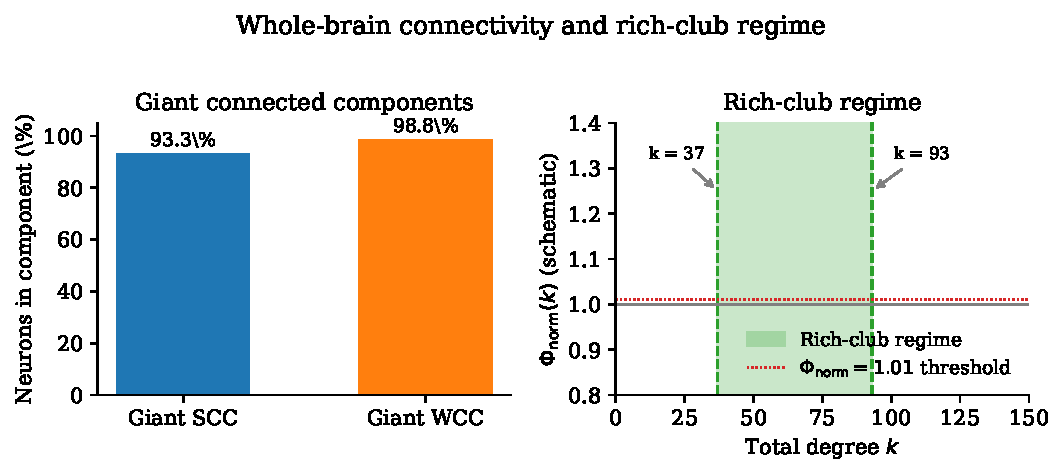
\includegraphics[width=0.95\linewidth]{figures/fig1_global.pdf}
\caption{Whole-brain connectivity and rich-club regime.
(a) Fraction of the $127{,}978$ neurons contained in the giant SCC
(93.3\%) and giant WCC (98.8\%) after thresholding at five synapses per
connection.
(b) The rich-club regime lies between total degree $k=37$ and $k=93$, the
range over which the normalized rich-club coefficient
$\Phi_{\mathrm{norm}}(k)$ exceeds the $1.01$ threshold relative to $100$
configuration null-model samples.}
\label{fig:global}
\end{figure}

\begin{figure}[htbp]
\centering
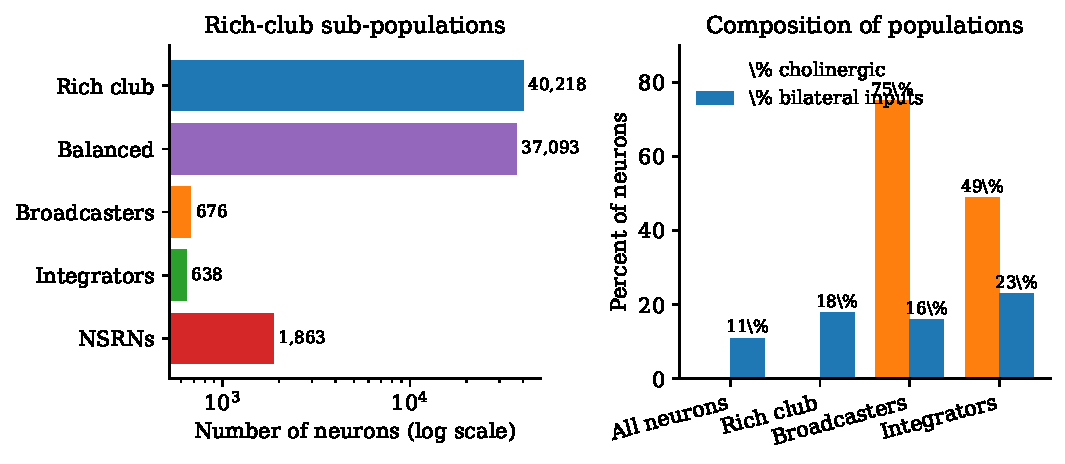
\includegraphics[width=0.95\linewidth]{figures/fig2_populations.pdf}
\caption{Rich-club sub-populations identified in the FlyWire connectome.
(a) Neuron counts for the rich-club ($n=40{,}218$), balanced
($n=37{,}093$), broadcaster ($n=676$), integrator ($n=638$), and
neuropil-specific highly reciprocal neuron (NSRN; $n=1{,}863$) populations.
(b) Cholinergic fraction (where reported) and fraction of neurons with
inputs in both hemispheres. Broadcasters are 75\% cholinergic;
integrators are 49\% cholinergic. Bilateral inputs: 11\% of all neurons,
18\% of rich-club neurons, 16\% of broadcasters, 23\% of integrators.}
\label{fig:populations}
\end{figure}

\begin{figure}[htbp]
\centering
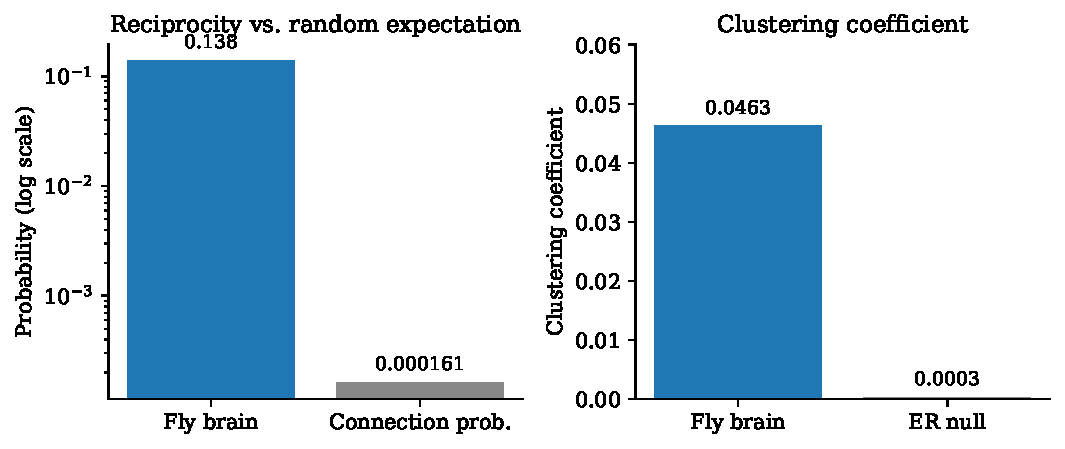
\includegraphics[width=0.9\linewidth]{figures/fig3_recip_clustering.pdf}
\caption{Reciprocity and clustering in the fly brain against random
baselines. (a) Whole-brain reciprocity ($0.138$) is much larger than the
brain-wide connection probability ($0.000161$) that sets the random pairing
baseline for reciprocity. (b) The global clustering coefficient ($0.0463$)
is two orders of magnitude larger than the matched-density ER null-model
value ($0.0003$).}
\label{fig:recip}
\end{figure}

\begin{figure}[htbp]
\centering
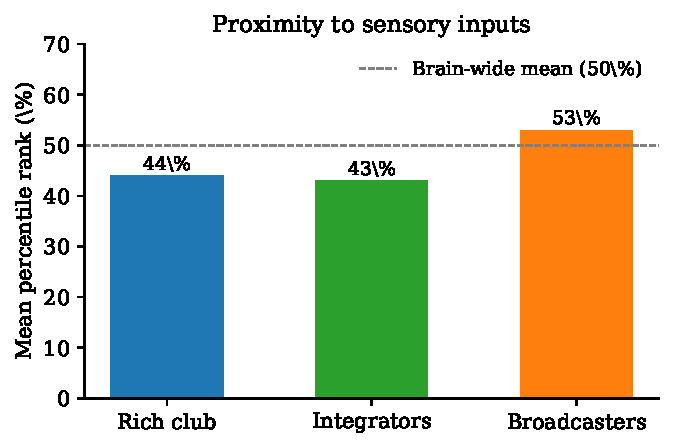
\includegraphics[width=0.6\linewidth]{figures/fig4_sensory_rank.pdf}
\caption{Mean percentile rank of rich-club sub-populations relative to the
full set of sensory inputs under the probabilistic information-flow model.
Rich-club neurons (44\%) and integrators (43\%) are closer than average to
sensory inputs, while broadcasters (53\%) are slightly farther. The
dashed line marks the brain-wide mean of 50\%.}
\label{fig:rank}
\end{figure}

\section{Discussion}

Our central claim is that the adult \textit{Drosophila} brain is a deeply
interconnected, pervasively recurrent, and non-hierarchical network
organized around a large distributed rich club rather than a small set of
hub neurons. The FlyWire connectome supports this claim at every level of
analysis we considered. A single giant SCC containing 93.3\% of neurons and a giant WCC
containing 98.8\% coexist with a rich club of $40{,}218$ neurons, or
approximately 30\% of the connectome, whose members preferentially span
the hemispheric midline and the central-brain--optic-lobe boundary.
Reciprocity ($0.138$) and clustering ($0.0463$) exceed all three null
models, and the distribution of three-node motifs is displaced away from
feedforward and toward recurrent configurations. These observations
together establish the fly brain as a densely recurrent substrate rather
than the shallow, hierarchical cascade that an intuitive sensory-to-motor
reading of the anatomy might suggest.

This architecture is particularly relevant in light of recent brain-wide
imaging experiments. Whole-brain recordings in behaving flies and in
other species have revealed distributed activity patterns that span many
neuropils during both sensory processing and simple
behaviors~\cite{mann2021coupling,ahrens2013whole}. A densely recurrent
connectome of the kind we report here provides a natural structural
substrate for such distributed dynamics: short average path lengths of
$4.42$ directed and $3.91$ undirected hops, together with a small-world
coefficient that far exceeds that of the \textit{C.\ elegans} connectome
($S_\Delta = 3.21$), make global communication kinetically feasible, while
the large rich club compensates for the anatomical bottlenecks posed by
the midline and the optic-lobe boundary. Consistent with this picture,
rich-club neurons were disproportionately bilateral (18\% compared with
11\% in the brain as a whole), and integrators and broadcasters were
preferentially close to one or more sensory modalities.

Our cross-species comparisons place the fly brain in context. The
reciprocity and clustering coefficient values reported here are
comparable to those reported for the hermaphrodite and male
\textit{C.\ elegans}~\cite{varshney2011structural,cook2019whole}, for
sub-volumes of larval zebrafish hindbrain~\cite{svara2022automated}, and
for L2/3 mouse visual cortex~\cite{song2005highly}, despite differences
in network size that span orders of magnitude. At the same time, the
relative size of the fly rich club---30\% versus the $\sim 4\%$ of the
worm~\cite{towlson2013rich}---is strikingly different, and the absence of
an out-degree-only rich club suggests that the fly network does not rely
on a small number of hub-like broadcasters. Rich-club organization was
previously inferred at the mesoscale for the human cortex and for
\textit{Drosophila} itself from projection
patterns~\cite{vandenheuvel2011rich,shih2015connectomics}; our
synapse-resolution analysis is consistent with those findings but also
shows that the fly rich club is distributed over tens of thousands of
neurons rather than concentrated in a handful of hubs, and that it is
chemically structured, with distinct excitatory broadcaster and
mixed-transmitter integrator populations nested inside it.

Several limitations of our analysis deserve emphasis. The neurotransmitter
predictions that underlie the chemical annotation of motifs are 94\%
accurate per neuron, and we have manually overwritten approximately
$1{,}600$ Kenyon cells that are known to be cholinergic despite
frequent misclassification; systematic errors in other neuron populations
without ground-truth labels cannot be ruled out. We have assumed Dale's
law and therefore ignore the known but still poorly quantified extent of
neurotransmitter co-transmission, as well as monoamines beyond dopamine,
octopamine, and serotonin and extrasynaptic signalling through
neuropeptides. Gap junctions are not captured by the synapse-based
reconstruction. The synapse-threshold choice of five synapses per
connection is conservative; although qualitative conclusions are robust
to threshold variation, the true network is almost certainly denser than
the one reported here, and topological statistics such as reciprocity and
motif frequency can shift with threshold. Finally, our cross-species
comparisons inherit the biases of the reference datasets, including the
sub-volume nature of the zebrafish and mouse reconstructions and
differences in synapse-detection pipelines across species.

Looking forward, the network statistics reported here are intended as a
quantitative baseline for future comparative connectomics. Additional
whole-brain datasets---further flies, the ventral nerve cord, and
non-insect species---will make it possible to distinguish conserved
architectural motifs from species- or individual-specific features. The
populations we highlight---attractor and repeller neurons, rich-club
members, broadcasters, integrators, and NSRNs---are concrete targets for
functional imaging and perturbation experiments that seek to link
structure to activity, and the lists of these neurons are shared
interactively through the FlyWire Codex. Combined with increasingly rich
mesoscale and whole-brain imaging in behaving
animals~\cite{mann2021coupling,ahrens2013whole}, the connectome-level
view we provide here should accelerate the transition from circuit-scale
hypotheses to brain-scale theories of computation.

\section{Conclusion}

We have presented a synapse-resolution network analysis of the first
whole-brain connectome of an adult \textit{Drosophila melanogaster}. The
brain is organized around a single giant connected component, a large
distributed rich club of $40{,}218$ neurons, and pervasive recurrent
motifs rather than hub-dominant or feedforward structure. Within the rich
club, chemically distinct broadcaster and integrator sub-populations and
neuropil-specific reciprocal neurons offer concrete circuit-level targets
for experimental and theoretical follow-up. The network statistics
reported here, together with the interactive neuron lists released
alongside this work, provide a baseline for comparison across individuals,
species, and developmental stages and establish the adult fly brain as a
reference point for connectome-scale network neuroscience.

\bibliographystyle{unsrtnat}
\bibliography{references}

\end{document}
